%
%  untitled
%
%  Created by Sergio on 2009-03-18.
%  Copyright (c) 2009 __MyCompanyName__. All rights reserved.
%
\documentclass[]{article}

% Use utf-8 encoding for foreign characters
\usepackage[utf8]{inputenc}
\usepackage[spanish]{babel}

% Setup for fullpage use
\usepackage{fullpage}

\usepackage{geometry}
% Uncomment some of the following if you use the features
%
% Running Headers and footers
%\usepackage{fancyhdr}

% Multipart figures
%\usepackage{subfigure}

% More symbols
%\usepackage{amsmath}
%\usepackage{amssymb}
%\usepackage{latexsym}

% Surround parts of graphics with box
\usepackage{boxedminipage}

% Package for including code in the document
\usepackage{listings}

% If you want to generate a toc for each chapter (use with book)
\usepackage{minitoc}

% This is now the recommended way for checking for PDFLaTeX:


%\newif\ifpdf
%\ifx\pdfoutput\undefined
%\pdffalse % we are not running PDFLaTeX
%\else
%\pdfoutput=1 % we are running PDFLaTeX
%\pdftrue
%\fi


\ifpdf
\usepackage[pdftex]{graphicx}
\else
\usepackage{graphicx}
\fi
\title{Final Computación gráfica}
\author{ Sebastián Arcila Valenzuela - Sergio Botero Uribe }

\date{\today}

\begin{document}
\pagestyle{empty}

\ifpdf
\DeclareGraphicsExtensions{.pdf, .jpg, .tif}
\else
\DeclareGraphicsExtensions{.eps, .jpg}
\fi

\maketitle


\section*{Instrucciones}
Para compilar el proyecto se debe ejecutar el 'Makefile' de la siguiente forma desde la línea de comandos:  \\ Para Linux:
	\begin{center}
	\begin{verbatim}
	$ make clean ; make
	$ ./raytracer} 
	\end{verbatim}
	\end{center}
Para Mac:
\begin{verbatim}
	$ make clean ; make mac
	$ ./raytracer 
\end{verbatim}
Para especificar un archivo 'input' de entrada se debe redireccionar el buffer de entrada de la siguiente forma:
\begin{verbatim}
	$ ./raytracer < input 
\end{verbatim}
\section*{Input}
El input debe contener las coordenadas del triángulo en sentido horario, de lo contrario no se verá correctamente la imágen.
%\newpage

\section*{Screenshot}


\begin{figure}%[ht] %  figure placement: here, top, bottom, or page
   \centering
   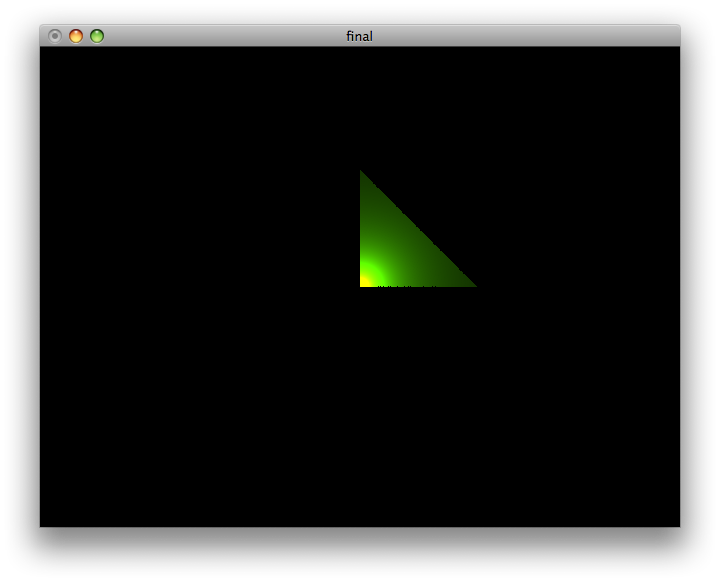
\includegraphics[width=6in]{Picture.png} 
   \caption{Screenshot del final en ejecución con el archivo de entrada 'input'}
   \label{fig:example}
\end{figure}

\bibliographystyle{plain}
\bibliography{}
\end{document}
